\setcounter{section}{20}

\section[Physics of Low-Dimension Systems: 2D]{\hyperlink{toc}{Physics of Low-Dimension Systems: 2D}}

\begin{itemize}
    \item \textbf{Graphene:} is single layer of atoms. they are 2D in the sense that the wavefunction is so confined to the plane of graphene and does not stick out at all.
    \item \textbf{2D electron gas (2DEG):} useful cause of their large mean free paths (low impurities), and high electron mobilities. 
    \begin{itemize}
        \item For MOS structures, at the semiC-insulator interface.
        \item For semiC heterostructures (remote dopants), 2DEG is formed at the interface between the 2 semiconductors.
    \end{itemize}
    \item \textbf{Density of State (DOS)for Free Electrons}:
    \begin{itemize}
        \item electrons not in a crystal (free in 3D) have a Fermi surface that is just a sphere. DOS is propto sqrt of E
        \item and in 2D Fermi surface is a circle. DOS is constant as E increases.
        \item in 1D Fermi surface is two points. DOS is propto 1/sqrt(E) as E increase. \textbf{van Hove singularity:} At energy E=0 electrons pile up (i.e. have a high DOS).
    \end{itemize}
    \item \textbf{Bands vs Sub-bands:} Sub bands are based on excited states
    \item Sub-bands for 1D:
    van-Hove singularities for each sub-band with density of state:
    \begin{equation}
        {g(E) = \frac{1}{\sqrt{E-En}}}
    \end{equation}
    \item Summary for all dimensions: 
    \begin{figure}
    \centering
    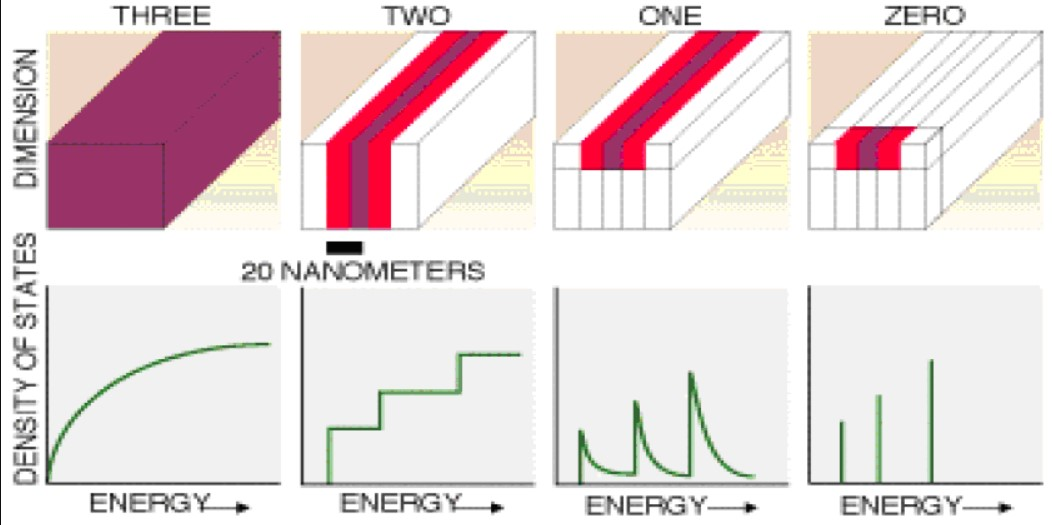
\includegraphics[width=0.75\linewidth]{Images/DOS.jpg}
    \caption{DOS}
    \label{fig:DOS}
    \end{figure}
    \item \textbf{Quantum Dotes:} 0D systems where the wavefunction of the system is the same size as the system. (for semiCs it can be tens of nm or the size of one atom).
    \item \textbf{Drude Model with a Magnetic field: Hall Effect:} Integer Quantum Hall effect. Expected classical linear increase in Resistance xy as perpendicular Bz field increases. 
    \item 2DEG in magnetic field at low temperatures so that QM effects can manifest nicely and instead we see linear increase only at small B increase but then we get a dramatically increasing staircase. Steps get bigger as we get to higher fields. Conductivity increases in equal steps.
    \item you expect resistance xx longitudinal to not change much. it starts out like this at low B field. But then everytime a jump happens in the hall resistance, a massive drop in Rxx occurs, going to to 0 ohms where it flows without resistance looking like a superconductor and then peaks that show insulating behaviour.
    \item 2DEG gets cyclotron motion with B-field (classical). From \textbf{Lorentz Force:}
    \begin{equation}
        \vec{F} = \frac{d\vec{p}}{dt} = q(\vec{v} \times \vec{B})
    \end{equation}
    \item Bohr-Sommerfeld quantization rule: number of wavelength along the trajectory must be integer. only discrete values of the trajectory radius are allowed. \textbf{Landau Levels:}
    \begin{equation}
        E_n = \hbar \omega_c (n+\frac{1}{2})
    \end{equation}
    \item Wave functions are smeared around classical orbits with:
    \begin{equation}
        r_n = l_B \sqrt{n} , \qquad l_B = \sqrt{\frac{\hbar}{m \omega_c}}
    \end{equation}
    \item where $l_B:$ magnetic length
    \item difference in classical and quantum here is that quantum has many different landau levels of radial SHO. each level has an enormous degeneracy (and is allowed because they don't overlap).  
    \item \textbf{Shubnikov-de Haas effect:} both Rxx and Rxy show oscillations at high magnetic field and low temp. each oscillation is a Fermi level pierced by a landau level. Oscillations allow to determine effective mass as well as scattering time. Efficient way to find parameters of 2DEG (magneto-transport studies).
    \item impurity may momentarily disrupt the forward propagation of the electron.
    \item Chiral edge channels: are these skipping electron edges
    \item composite picture of \textbf{FQHE}
    
    
\end{itemize}
